%----------------------------------------------------------------------------------------
%	OPACITY MEASURES
%----------------------------------------------------------------------------------------

\section{Opacity measurements {\color{blue} Juan $\&$ Laurence}}
\label{se:opacity_correction}

%{\bf copy from the 'Instru' paper}

%\begin{figure}[ht]
%\begin{center}
%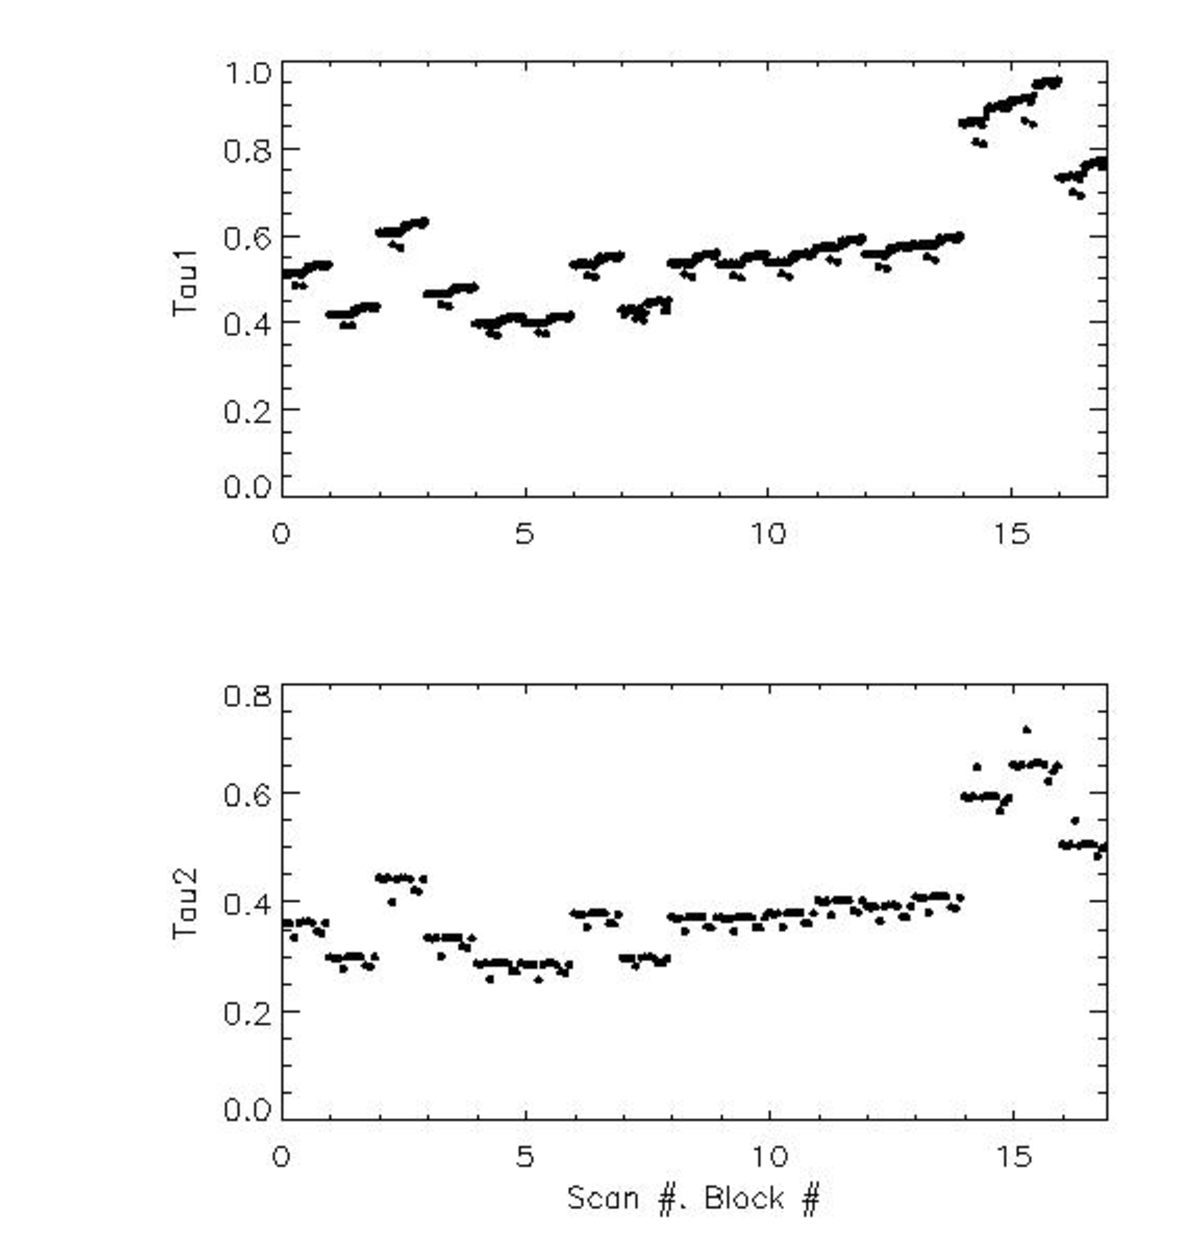
\includegraphics[scale=0.8]{Figures/test_allskd_N2R10v3commiss2.pdf}
%\caption{Atmospheric opacity as measured from the NIKA2 data 
%at 260 (top) and 150\,GHz (bottom) during N2R10
%commissioning campaign. Each block of 40 KIDs gives an independent estimate of
%the opacity value for each skydip scan (the integer abscissae). The block
%number is the decimal value of the abscissae.
%\label{fig:taumeas_paper}}
%\end{center}
%\end{figure}

%\begin{figure}[ht]
%\begin{center}
%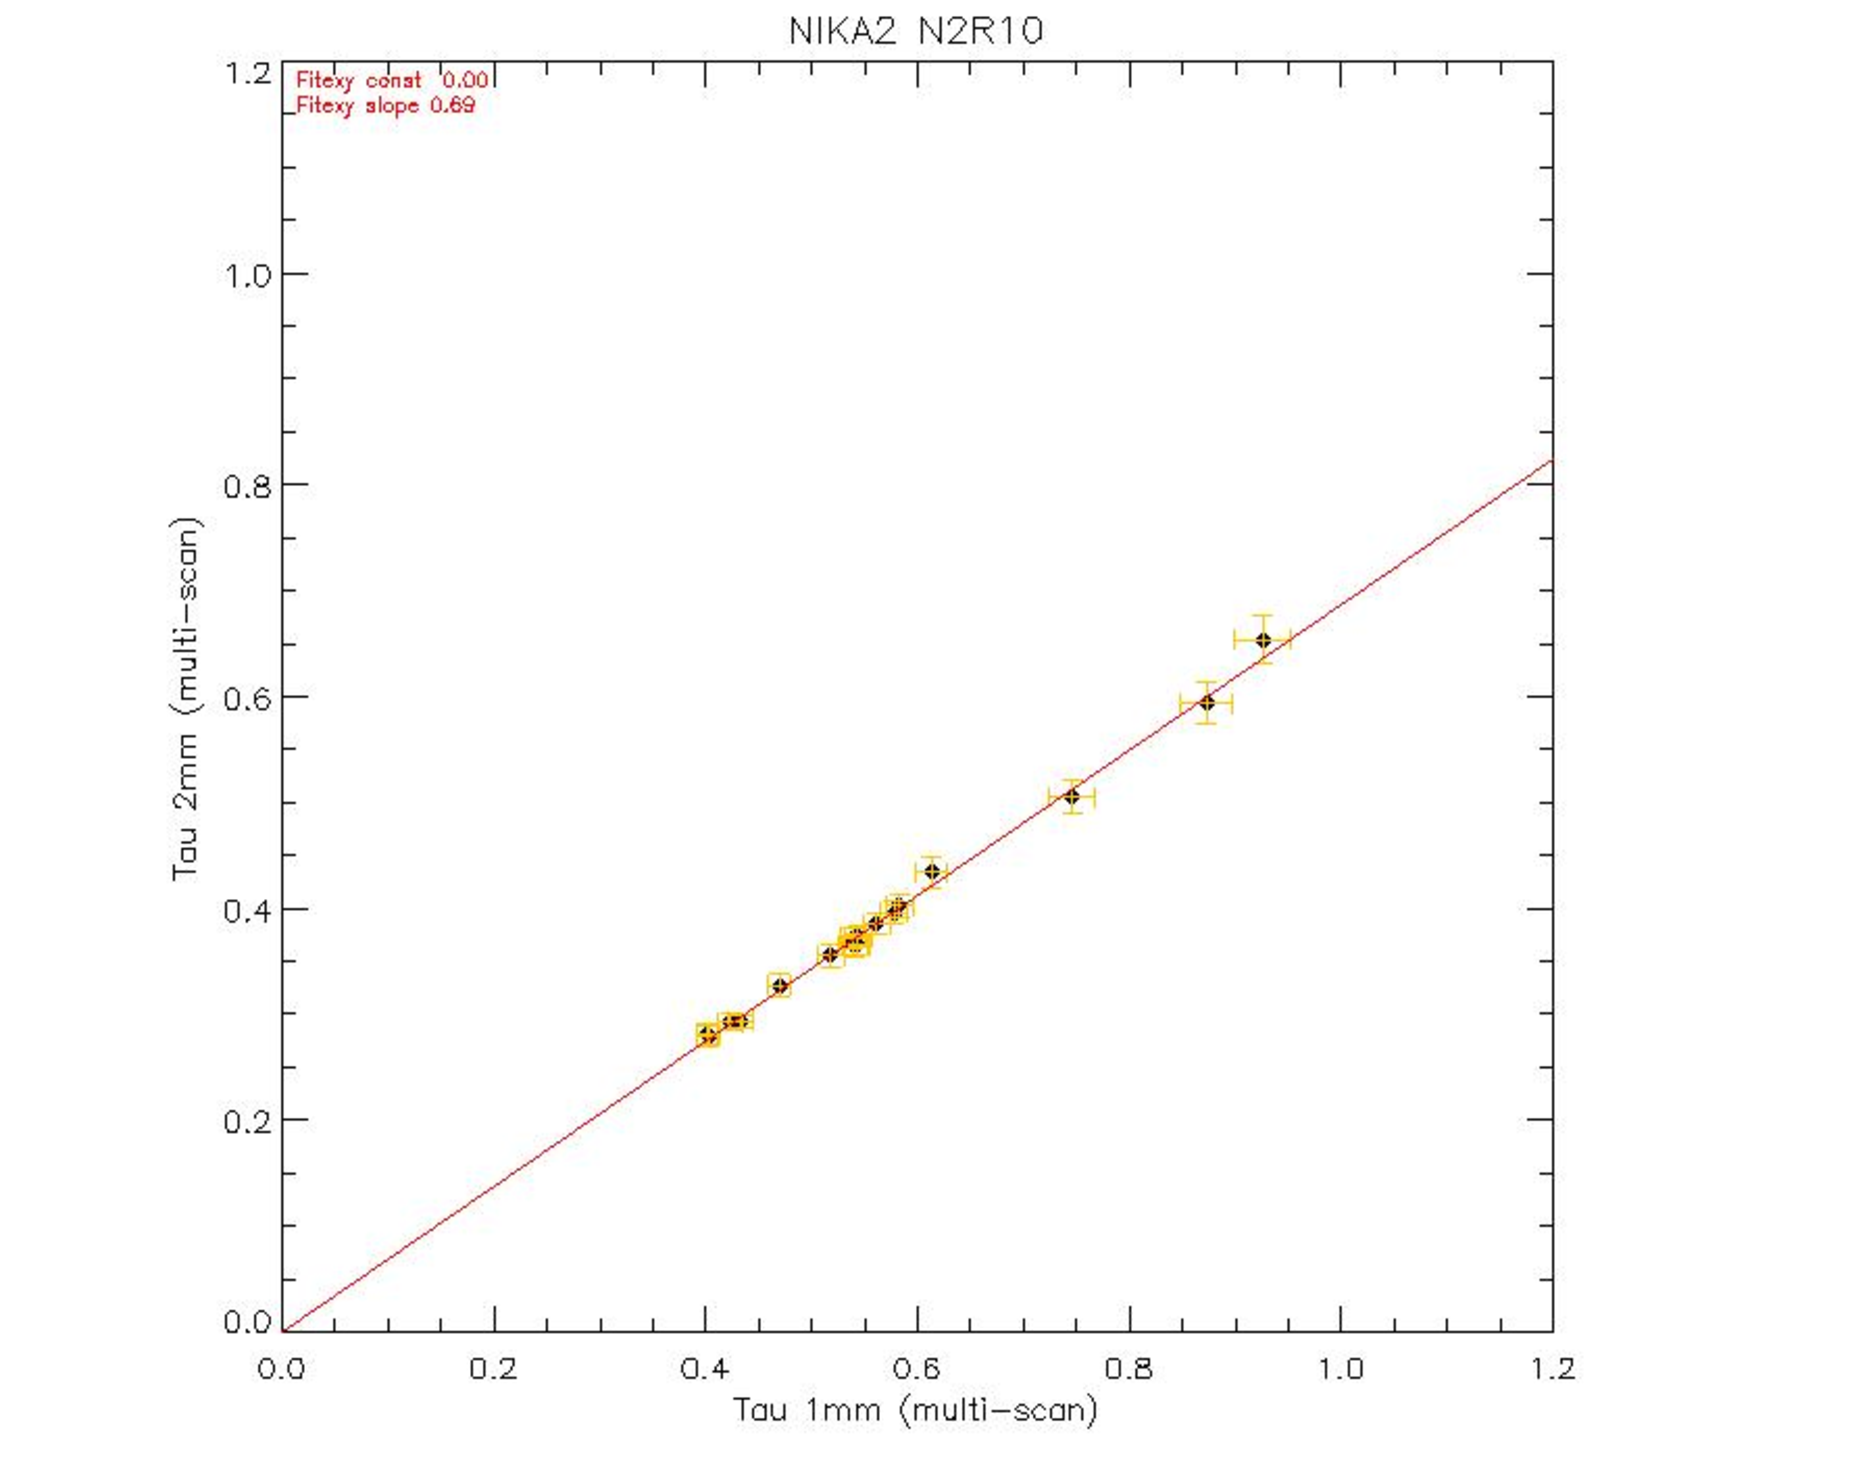
\includegraphics[scale=0.8]{Figures/test_allskd_N2R10v2commiss1.pdf}
%\caption{Atmospheric opacity as measured from the NIKA2 data 
%at 260 and 150\,GHz during N2R10
%commissioning campaign. The error bars are in fact dispersion of the deduced
%opacities between blocks of 40 KIDs.
%\label{fig:taumeas_paper}}
%\end{center}
%\end{figure}

We observe that the skydip-fitted $\tau$ values are, as expected, common
between different detectors of the same array. By comparing the results of different skydips, we
have verified experimentally that the coefficients $C_0$, $C_1$ are stable,
within the fit errors, on very long time scales within a cooldown cycle. The
coefficients can thus be applied to the whole observing campaign in order to
recover the opacity of each scan.


% \noindent {\bf FM : a figure would help to convince the reader that it is stable on lng time
% scale, which is a key point.}\\ FXD: I will do that figure


\begin{figure}[ht]
\begin{center}
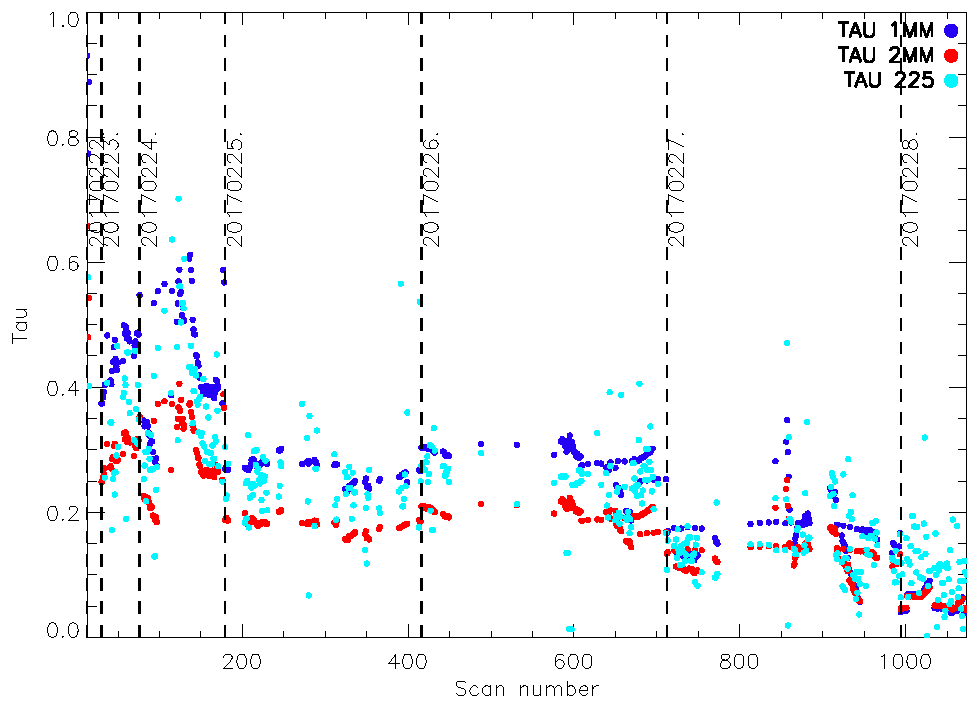
\includegraphics[scale=0.8]{../../../Paper_NIKA2_Technical/opacity_evol_run22.pdf}
\caption[Zenith opacity monitoring during N2R9]{Atmospheric opacity as measured from the IRAM 225\,GHz taumeter
(cyan), and from the NIKA2 data at 150 (red) and 260\,GHz (blue) during N2R9
commissioning campaign (Feb. 2017). We stress the fact that the IRAM 225\,GHz
taumeter data is not used for the atmospheric correction and is plotted here
just for comparison.
  \label{fig:taumeas_paper}}
\end{center}
\end{figure}


\begin{figure}[ht]
\begin{center}
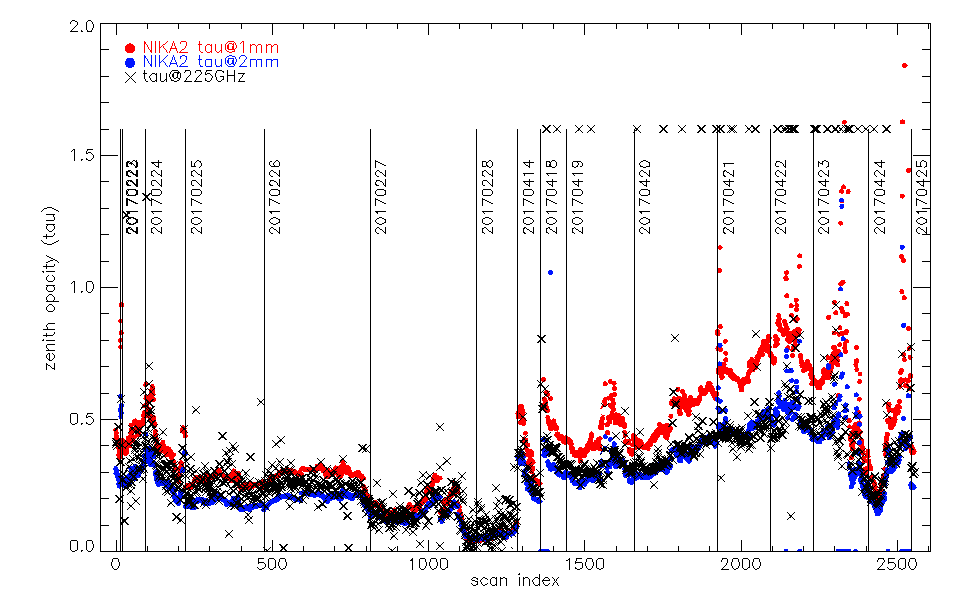
\includegraphics[width=\linewidth]{Figures/opacity_vs_index_N2R9_N2R10.png}
\caption[Zenith opacity monitoring during N2R9 and N2R10]{Atmospheric opacity as measured from the IRAM 225\,GHz
  taumeter (black crosses), and from the NIKA2 data at 150 (red) and 260\,GHz (blue) during 
  N2R9 and N2R10 commissioning campaigns.  We stress the fact that the IRAM 225\,GHz taumeter data is not used for the atmospheric correction and is plotted here just for comparison.
  \label{fig:taumeas}}
\end{center}
\end{figure}


In Fig.~\ref{fig:taumeas} {\bf(and Fig.~\ref{fig:taumeas_paper} of
  \cite{Adam18}) } we present the evolution of the NIKA2 in-band
opacities for all the 'OTF' scans (about 1300 scans per runs) of the
N2R9 run held in February and the N2R10 run in April 2017. These are
compared to the IRAM tau-meter values. We observe an agreement on the global trend between the IRAM tau-meter opacity (225 GHz) and the NIKA2 values. These latter show, however,
a smaller dispersion (less than one percent).


